\subsection{Motivation}
Mit der steigenden Zahl an Nachrichten aus immer mehr Kanälen steigt auch der Aufwand,
diese zu bewerten. Als eine Möglichkeit bietet es sich deshalb ab,
Nachrichten automatisiert durch Computer vorab bewerten zu lassen.
Anstatt einen Bewertungs-Algorithmus blind sämtliche Nachrichten eines Kanals
oder einer Quelle bewerten zu lassen, können Nachrichten vorher auch thematisch gesammelt
und gespeichert werden.

\subsection{Projektziel}
Das Ziel dieses Projekts ist die Konzeption und Erstellung eines Newsboards zum Speichern
gesammelter Nachrichten und deren Bewertungen. Das eigentliche Sammeln
und Bewerten der Nachrichten geschieht durch externe Module,
die über eine Schnittstelle mit dem Newsboard kommunizieren.

Darüber hinaus soll das Newsboard auch eine grafische Oberfläche enthalten,
mit der die enthaltenen Nachrichten und deren Bewertungen eingesehen werden können.
%Außerdem sollte eine rudimentäre Administrations-Funktion verfügbar sein.
Aus diesen Anforderungen kann das in Abbildung \ref{fig:use-cases} dargestellte
Minimalset an Anwendungsfällen abgeleitet werden.

\begin{figure}[h]
	\centering 
	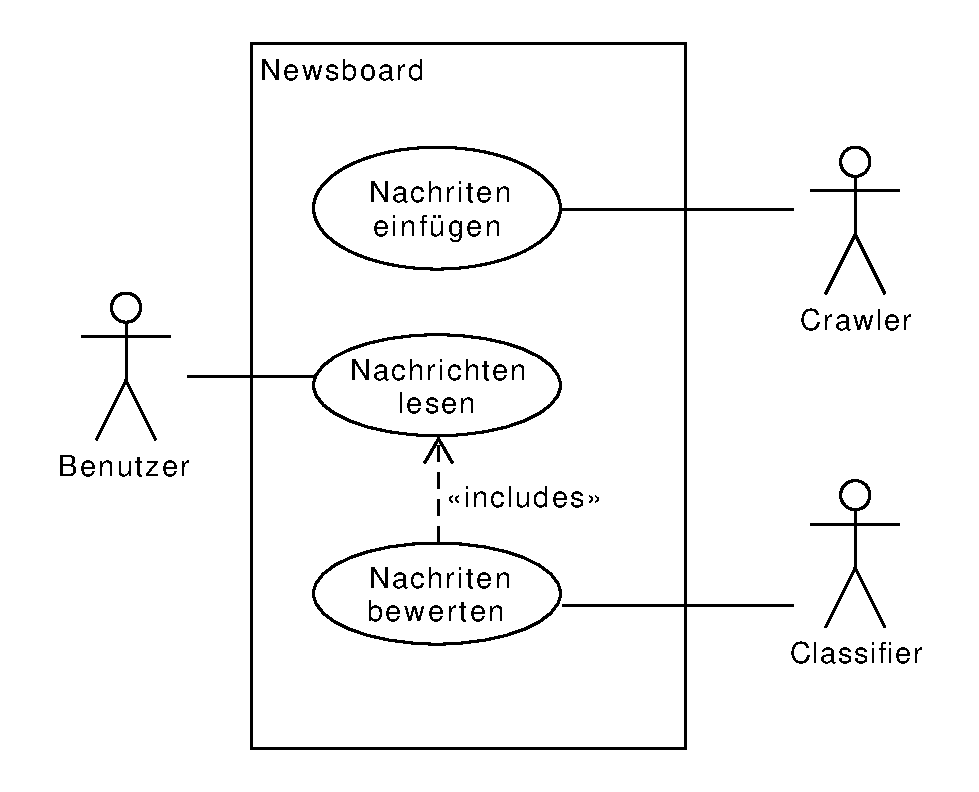
\includegraphics[scale=0.75]{assets/use-cases.pdf}
	\label{fig:use-cases}
	\caption{Anwendungsfälle}
\end{figure}

Das Newsboard soll verwendet werden, um Nachrichten zu sammeln und zu bewerten,
welche die Fachhochschule Bielefeld betreffen. Darüber hinaus soll es
als möglichst praxisnahe Möglichkeit dienen, im Module Intelligente Systeme entwickelte
Crawler- und Bewertungsmodule zu verwenden.
